\documentclass{article}
% \usepackage[utf8]{inputenc}
\usepackage{layout}

% ===-===-===-===-===-===-===-===-===-
% Font >>>
\usepackage[fontsize=9.5pt]{fontsize}
\renewcommand{\sfdefault}{phv} % Arial
\renewcommand{\familydefault}{\sfdefault}
% Font <<<
% ===-===-===-===-===-===-===-===-===-

% ===-===-===-===-===-===-===-===-===-
% Colors definitions >>>
\usepackage{xcolor}
\definecolor{titlecolor}{RGB}{60,100,100}
% Colors definitions <<<
% ===-===-===-===-===-===-===-===-===-

% ===-===-===-===-===-===-===-===-===-
% Header commands >>>
\newcommand{\abstracttitle}[1]{
\begin{center}{
    \textcolor{titlecolor}{\fontsize{15pt}{16pt}{\textbf{#1}}}
    }\vspace{0pt}
\end{center}}

\newcommand{\authors}[1]{
\begin{center}{
    \fontsize{11pt}{12pt}\textbf{#1}
    }\vspace{-8pt}
\end{center}}

\newcommand{\affiliation}[1]{
\begin{center}{
    \fontsize{11pt}{12pt}\textit{#1}
    }\vspace{-8pt}
\end{center}}

\newcommand{\auth}[2][1]{#2$^{#1}$}
\newcommand{\affi}[2][1]{$^{#1}$#2}

\newcommand{\keywords}[1]{{
    \small{\underline{Keywords:} #1}
    }
    \vspace{4pt}
}
% Header commands <<<
% ===-===-===-===-===-===-===-===-===-

% ===-===-===-===-===-===-===-===-===-
% Margins settings >>>
\setlength{\voffset}{-10mm}
\setlength{\topmargin}{0pt}
\setlength{\headheight}{12pt}
\setlength{\headsep}{8mm}
\setlength{\oddsidemargin}{0pt}

% \setlength{\hoffset}{-3mm}
\setlength{\textheight}{220mm}
\setlength{\textwidth}{165mm}

\setlength{\marginparwidth}{0pt}
\setlength{\marginparsep}{0pt}

% Margins settings <<<
% ===-===-===-===-===-===-===-===-===-

% ===-===-===-===-===-===-===-===-===-
% Caption set up >>>
\usepackage{caption}
\captionsetup[figure]{font={it,small},name={Fig.},labelsep=endash, justification=centering}
% Caption set up <<<
% ===-===-===-===-===-===-===-===-===-

% ===-===-===-===-===-===-===-===-===-
% Paragraphs set up >>>
\setlength{\parindent}{0mm}
\setlength{\parskip}{1.85mm}

\setlength\intextsep{1.5mm}
% Paragraphs set up <<<
% ===-===-===-===-===-===-===-===-===-

% ===-===-===-===-===-===-===-===-===-
% Page numbering >>>
\pagenumbering{gobble}
% Page numbering <<<
% ===-===-===-===-===-===-===-===-===-

% ===-===-===-===-===-===-===-===-===-
% Headers >>>
\usepackage{fancyhdr}
\usepackage{graphicx}
\usepackage[absolute,overlay]{textpos}

\renewcommand{\headrulewidth}{0pt}

\pagestyle{fancy}
\lhead{\begin{picture}(0,1mm)
{
\includegraphics[height=10mm,width=55mm]{logo.png}}
\end{picture}
}
\rhead{\bf{PECS Research Conference 2022}}
% Headers <<<
% ===-===-===-===-===-===-===-===-===-

% ===-===-===-===-===-===-===-===-===-
% Footer >>>
% !!!!!!! Please change this section according to your topic and type of presentation !!!!!!

\pagestyle{fancy}
\lfoot{Topic \# ...}

\pagestyle{fancy}
\rfoot{Oral or Poster (please specify)}
% Footer <<<
% ===-===-===-===-===-===-===-===-===-

% ===-===-===-===-===-===-===-===-===-===-===-===-===-===-===-===-===-===-
\begin{document}

\abstracttitle{Title Calibri, 16 pt, bold, (R=60 G=100 B=100)}
% Please provide a list of authors below. Use \auth for every author: \auth[affiliation number]{Author Name}
% Please update the affiliation list accordingly.
\authors{
    \auth[1]{Author Aname}, 
    \auth[2]{Author Bname}
}

% \affi[affiliation number]{Institution name}
\affiliation{
    \affi[1]{Affiliation A}; 
    \affi[2]{Affiliation B};
}

\keywords{keyword1, keyword2}

% ===-===-===-===-
% Main text:

1. The body of the abstract must be composed using calibri 10 pt, example: References should be indicated with numbers and respect the proposed formatting [1]. Here is an example text: Digital Microfluidics (DMF) [2] is a technique facilitating automated, discrete, sequential manipulation of microlitre-size droplets. DMF has been described as a new paradigm for microfluidics in general and Lab-on-a-Chip applications in particular [3].

Droplets (Fig. \ref{fig:main_figure}) are precisely manipulated thereby facilitating automated, miniature version of ‘bench (bio)chemistry’ including self-contained sequential processes possibilities otherwise limited or restricted when employing traditional continuum microfluidics.

\begin{figure}[h!]
\centering
  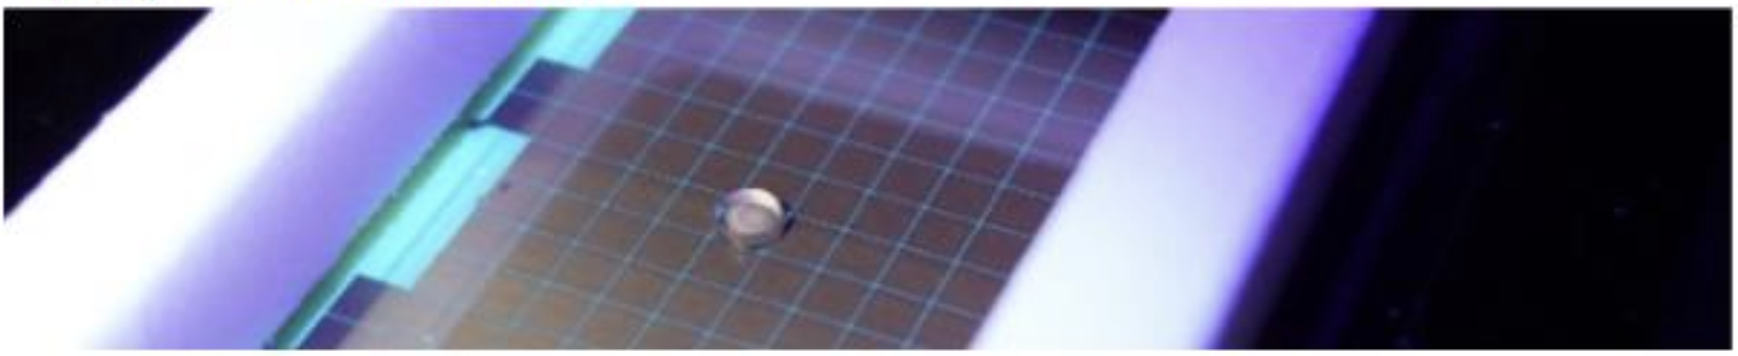
\includegraphics[width=\linewidth]{main_figure.png}
  \caption{
    Example figure – calibri 9, italic
  }
\label{fig:main_figure}
\end{figure}

2. The context of the research work, the objectives, the methodology, the main results and conclusions must be clearly mentioned in the abstract to facilitate a smooth review process.

3. The main results and conclusions must be supported with a single figure which can be composed of multiple subfigures. The figure caption must be composed using {\small 9 pt Calibri}.

\textbf{4. The entire abstract (including text, figure, references) must not exceed one A4 page with the specified typesetting.}

\textbf{5. Appropriate References} must be provided References must be numbered sequentially in their order of appearance as [1], [2]…

The reference list calibri 9 pt must be provided at the end as: [1] Author 1 Name, Author 1 Initial(s), \textit{et al.} (date) Journal \textbf{Volume}(issue) page

6. In the footer of this document please indicate the topic under wish you want your research to be presented and indicate your preference of poster or oral presentation. 

\textbf{7. A word version of the abstract must be sent via email to l.coudron@herts.ac.uk Before the specified deadline}

\textbf{The subject of the email should be: [PECS Conf] + abstract title}

\textbf{Please make sure the above is used when sending your abstract otherwise it may be overlooked }


% ===-===-===-===-
% References:
\vspace{3mm}
\textbf{References}

[1] Author 1 Name, Author 1 Initial(s), \textit{et al.} (date) Journal \textbf{Volume}(issue) page

[2] Cho, S.K. \textit{et al.} (2003) Journal of microelectromechanical systems \textbf{12}(1) 70

[3] Abdelgawad, M. \textit{et al.} (2009) Advanced Materials \textbf{21}(8) 920
% ===-===-===-===-


% ===-===-===-===-===-===-===-===-===-===-===-===-===-===-===-===-===-===-
\end{document}
